\begin{flushleft}
	If your system is getting stuck during system boot, you can troubleshoot the system by booting it into rescue or emergency mode:
\bigskip
\begin{itemize}
	\item Append either \textbf{systemd.unit=rescue.target} or \textbf{systemd.unit=emergency.target} to the kernel command line to boot the system into a  rescue or emergency shell instead of starting normally. 
	\item Both of these shells require the root password. 
	\item The \textbf{emergency.target} keeps the root file system mounted read-only.
	\begin{figure}[h!]
		\centering
		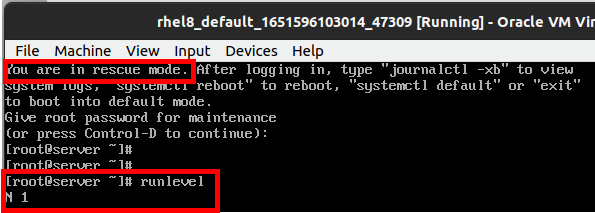
\includegraphics[scale=.6]{content/chapter1/images/emer.png}
		\caption{Sample output}
		\label{fig:free_h_s_2_3}
	\end{figure}
	
	\item The \textbf{rescue.target} waits for sysinit.target to complete first so that more of the system will be initialized, for example, logging, file systems, etc. 
	\begin{figure}[h!]
		\centering
		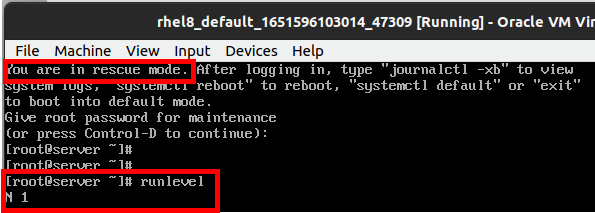
\includegraphics[scale=.6]{content/chapter1/images/rescue2.png}
		\caption{Sample output}
		\label{fig:free_h_s_2_4}
	\end{figure}
	
	\item Exiting from these shells will continue with the regular boot process.
\end{itemize}
\end{flushleft}

\newpage